\documentclass[tikz,border=2pt]{standalone}
\renewcommand{\familydefault}{\sfdefault}
\usetikzlibrary{arrows.meta,calc,positioning}
\tikzset{every picture/.style={line width=1pt, >=Stealth},
         hl/.style={fill=black, fill opacity=0.12, text opacity=1}}
\usepackage{amssymb}
\begin{document}
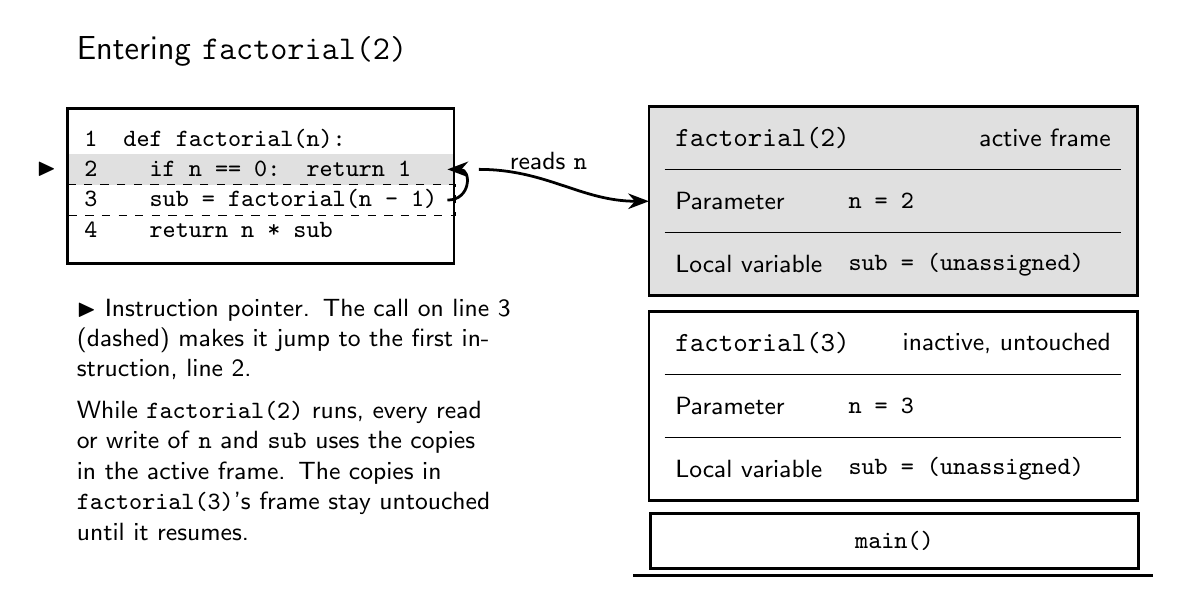
\begin{tikzpicture}[frame/.style={draw, minimum width=6.2cm, minimum height=0.7cm, font=\ttfamily\small},
    code/.style={draw, font=\ttfamily\small, inner sep=6pt}, small/.style={font=\small}]
  \node[anchor=west, font=\large] at (0, 1.1) {Entering \texttt{factorial(2)}};
  \node[code, anchor=north west] (code) at (0, 0.4) {%
    \begin{tabular}{@{}r@{\quad}l@{}}
      1 & def factorial(n): \\
      2 & \ \ if n == 0: return 1 \\
      3 & \ \ sub = factorial(n - 1) \\
      4 & \ \ return n * sub
    \end{tabular}};
  % Line 2 is where the instruction pointer jumps to; line 3 (dashed) made the call.
  \fill[black, fill opacity=0.12] ([yshift=-0.6cm]code.north west) rectangle ([yshift=-0.99cm]code.north east);
  \draw[thin, dashed] ([yshift=-0.99cm]code.north west) rectangle ([yshift=-1.38cm]code.north east);
  \node[small] at ([shift={(-0.25, -0.795)}]code.north west) {$\blacktriangleright$};
  \draw[->] ([shift={(-0.1, -1.185)}]code.north east) to[out=0, in=0, looseness=2] ([shift={(-0.1, -0.795)}]code.north east);
  \node[anchor=north west, small, text width=5.8cm] at ([yshift=-0.3cm]code.south west)
    {$\blacktriangleright$ Instruction pointer. The call on line 3 (dashed) makes it jump to the first instruction, line 2.\\[4pt]
     While \texttt{factorial(2)} runs, every read or write of \texttt{n} and \texttt{sub} uses the copies in the active frame.
     The copies in \texttt{factorial(3)}'s frame stay untouched until it resumes.};

  % The stack: the active frame on top, the caller's frame below it.
  \foreach \y/\name/\note/\n/\s in {0.4/factorial(2)/active frame/2/hl, -2.2/factorial(3)/{inactive, untouched}/3/} {
    \draw[\s] (7.4, \y) rectangle (13.6, \y - 2.4);
    \node[anchor=west, font=\ttfamily] at (7.6, \y - 0.4) {\name};
    \node[anchor=east, small] at (13.4, \y - 0.4) {\note};
    \draw[thin] (7.6, \y - 0.8) -- (13.4, \y - 0.8);
    \node[anchor=west, small] at (7.6, \y - 1.2) {Parameter};
    \node[anchor=west, font=\ttfamily\small] at (9.8, \y - 1.2) {n = \n};
    \draw[thin] (7.6, \y - 1.6) -- (13.4, \y - 1.6);
    \node[anchor=west, small] at (7.6, \y - 2) {Local variable};
    \node[anchor=west, font=\ttfamily\small] at (9.8, \y - 2) {sub = (unassigned)};
  }
  \node[frame, anchor=north west] at (7.4, -4.75) {main()};
  \draw (7.2, -5.55) -- (13.8, -5.55);
  \draw[->] ([shift={(0.3, -0.795)}]code.north east) to[out=0, in=180] node[above, small, pos=0.4] {reads \texttt{n}} (7.4, -0.8);
\end{tikzpicture}
\end{document}
